%!Mode::"TeX:UTF-8"

\documentclass[12pt, a4paper]{book}

\usepackage{CJKutf8}
\usepackage[unicode={true}]{hyperref}
\usepackage{color}
\usepackage{graphicx}

\title{\textbf{The Legendary Romance of Seven Hulus}}
\author{Executive Cabinet of Xiao-Ming Kingdom}
%\date{}

\begin{document}
\begin{CJK}{UTF8}{gbsn}

    \maketitle
    \clearpage
    \thispagestyle{empty}

    \frontmatter
    
    \vspace*{50 mm}
    \begin{center}
    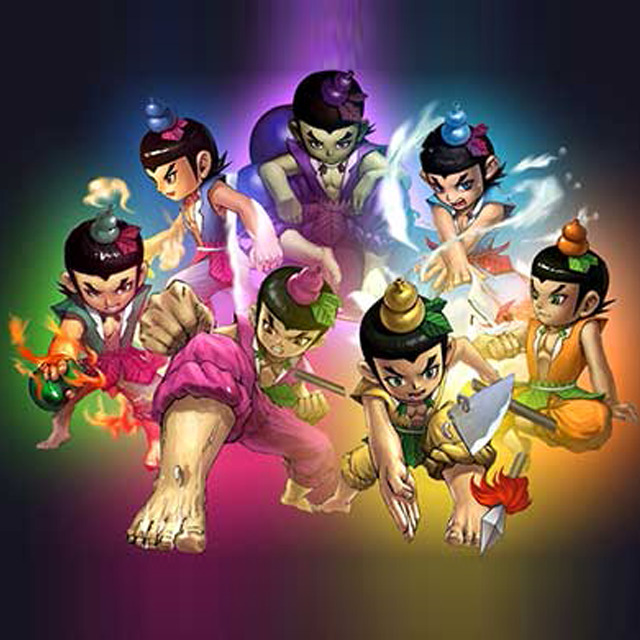
\includegraphics[width=0.6\textwidth]{figure/hulu.png}
    \end{center}

    %\include{preface/intro}
    %!Mode::"TeX:UTF-8"

\chapter{Preface}

谨以此纪念孙晓峰葫芦娃断浆行舟的昂扬青春。

    \chapter{Acknowledgement}

谨对小明王朝执行内阁全体成员为本书提供的宝贵史料致以诚挚的谢意。


    \chapter{楔子  穿山甲误走蛇蝎怪 盘古氏结缘葫芦藤}
    
    \tableofcontents

    \mainmatter

    %%!Mode::"TeX:UTF-8"

\chapter[历酷暑四字建班号 流火季七葫聚帝都]{历酷暑四字建班号\\\quad流火季七葫聚帝都}

没内容,你咬我啊

    %\chapter[着绿装众娃皆做火 披迷彩夜探北沙窝]{着绿装众娃皆做火\\\quad披迷彩夜探北沙窝}

没内容,你咬我啊


    \chapter{武曲星再起关中地 赤葫芦伟力撼京营}
    
    没内容就是没内容。

    \chapter{修杨树辽东王出世 上镜头橙葫芦初名}
    
    没内容你咬我啊。
    
    \chapter{关外雪冻碎钢筋骨 关内风吹干黄葫芦}

    \chapter{军训场佳偶初相会 火葫芦观星撩良辰}

    \chapter{强迫症病发残足趾 水葫芦玩火焚自身}

    \chapter{浪里白条萌相毕露 行踪无影蓝娃狐行}

    \chapter{盘天象处女拱红日 收万物紫娃覆雨云}

    \chapter{奥运年未及观奥运 流沙河红黄战流沙}

    \chapter{班封零复始新万物 五葫芦聚首紫荆园}

    \chapter{行万里赤葫芦北去 读万卷黄葫芦留燕}

    \chapter{历答辩众葫芦称导 经风雪赤葫芦归京}

    \chapter{四二一七葫芦聚义 东西北众诸侯会师}

    \chapter{带军训蓝娃改送水 管熊宝水娃Angry}

    \chapter{无制服紫娃怒隐身 随拉练三娃摔破膝}

    \chapter{三班倒二娃观八面 一横心大娃战通宵}

    \chapter{军训过再逢一二九 水葫芦灌水强出头}

    \chapter{水娃暴饮水下如牛 火娃添杯火上浇油}
    
    \chapter{建王朝众葫芦组阁 称学士水葫芦秉政}
    
    \chapter{力无穷晋位指挥使 撩良辰职司钦天监}
    
    \chapter{恋百味二娃掌礼部 育后生七娃监国子}
    
    \chapter{悬明镜六娃卿大理 爱唠叨三娃赴六科}
    
    \chapter{秀恩爱少卿出新招 长颈鹿化身大白兔}
    
    \chapter{百色芒果北上帝都 留守葫芦心念二娃}
    
    葫芦三年七月十一日,礼部侍郎娃二八百里速递桂地芒果入京。看守内阁文员,户科给事中娃三收讫,分送驻京阁属,俱喜而歌,以为消暑佳品。
    
    \chapter{酒娃潜水九米九九 夜游南海白浪滔滔}
    
    葫芦三年七月十六日,大学士袁志刚同志视察南海建设情况,亲自潜入海底指导虾兵蟹将的生产生活,奋力探索、细致入微\marginpar{\color{blue}据传闻,大学士袁志刚因水下光线条件有限,探索过程中误触女同志,被殴血流;大学士自称为遇到未名生物蛰刺所致。}、通宵达旦。入夜,大学士与随从仍畅游南海,并细数千百年来诸多深海怪物与意外事件,惟妙惟肖、绘声绘色,从人甚恐,遂于次日凌晨登陆,返回驻跸之地。
    
    \chapter{帝都暴雨水娃远观 滴滴出行火娃炫富}
    
    葫芦三年七月廿日,帝都暴雨,水漫金山,鞋履鱼行,衣衫水浸。是时,雨神下凡、东海龙王、大学士袁于桂地视察,发布声明不对此次事件负责。驻京留守、钦天监正、四娃冰洁因产学联络工作,以软件应用滴滴出入宫禁,日费百金之巨。
    
    大学士袁赞钦天监正曰:“让你昨天秀工资秀看剧欺负我,哼。”
    
    \chapter{手机桌面争奇斗艳 上善若水浪得飞起}

    葫芦三年七月廿一,内阁议事,共 show 手机 desktop。

    大学士袁首 show 女孩图片,以为萌,宜桌面。

    \begin{center}
        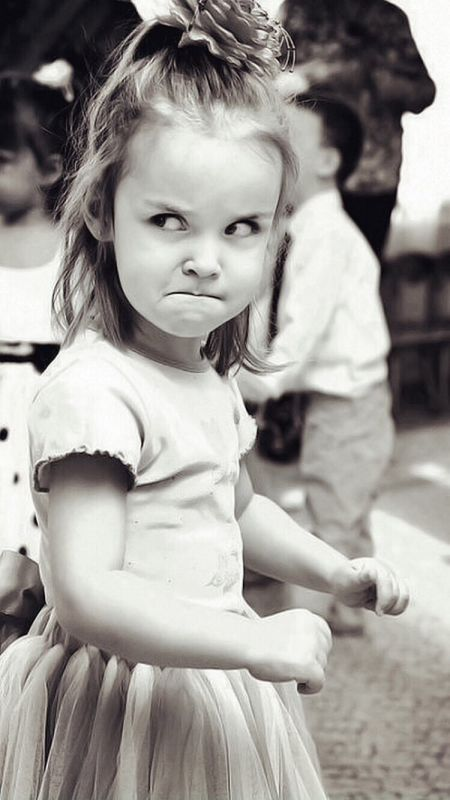
\includegraphics[height=0.3\textheight]{./figure/desktop-0.jpg}
    \end{center}

    国子监监正不以为然,show 美食图片,宜缓解工作之压力,提醒饮食之规律,抚慰加班之心灵。

    \begin{center}
    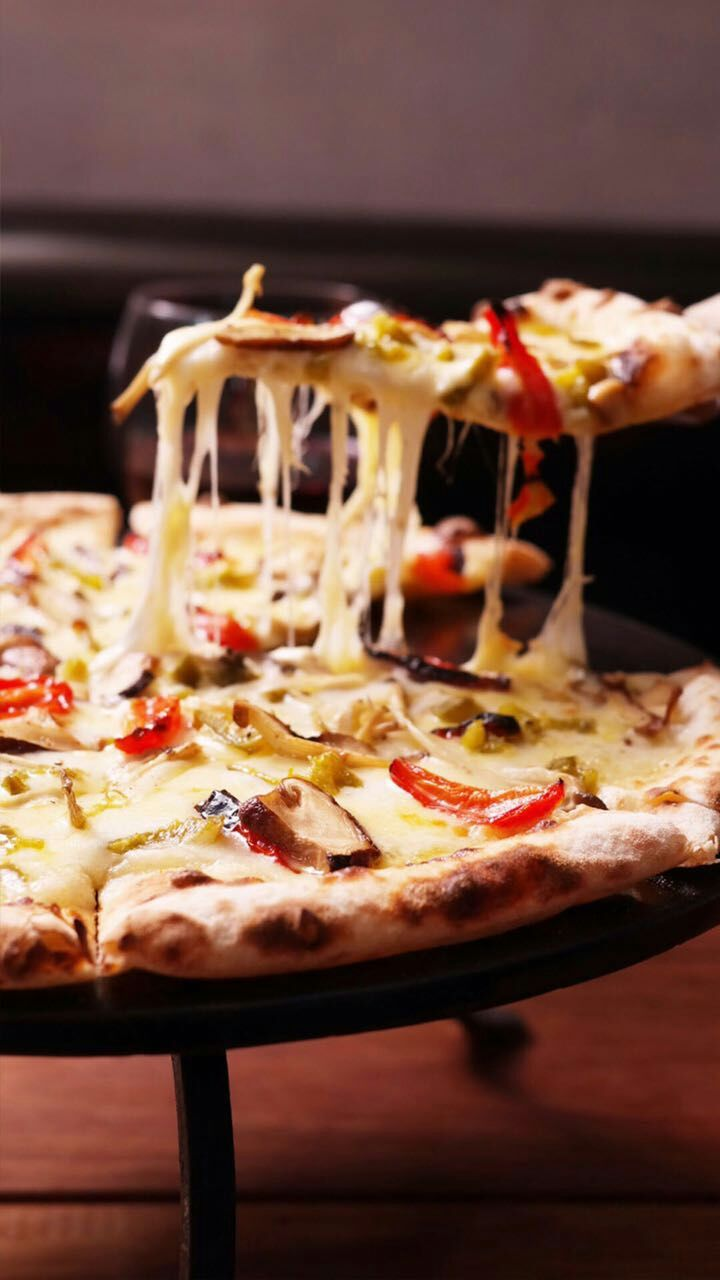
\includegraphics[height=0.3\textheight]{./figure/desktop-1.jpg}
    \end{center}

    大学士袁叹曰,理想很丰满,现实很骨感,show 其手机桌面,众 APP 分门别类于各文件夹下,名之为,上善若水。

    \begin{center}
    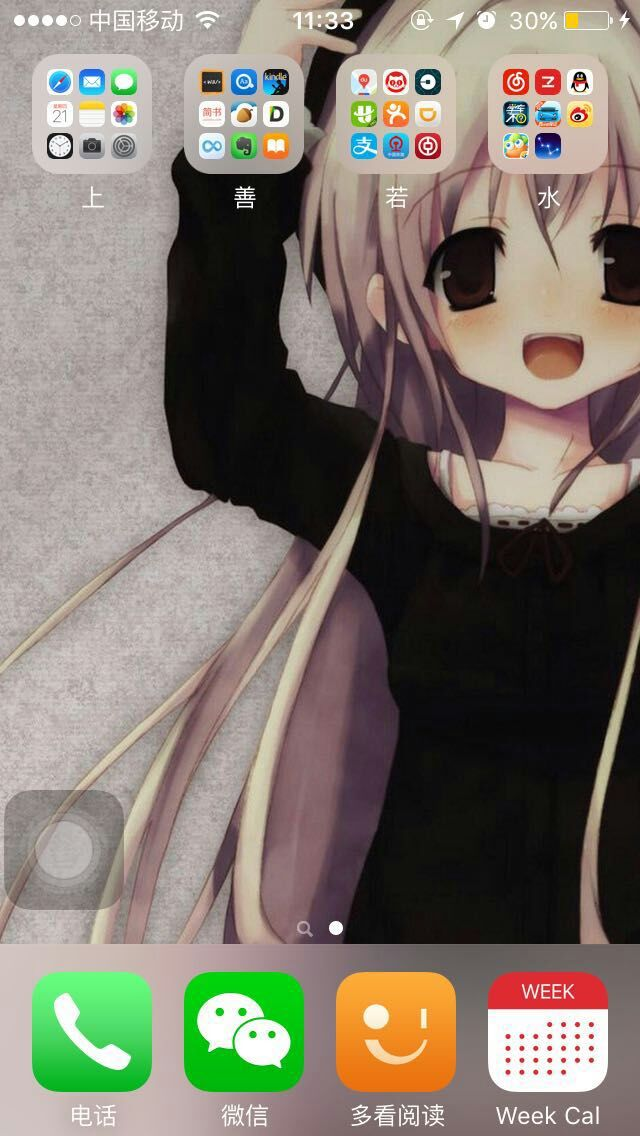
\includegraphics[height=0.3\textheight]{./figure/desktop-2.jpg}
    \end{center}

    户科给事中刘赞之,并 show 其手机桌面,以为大道至简。

    \begin{center}
    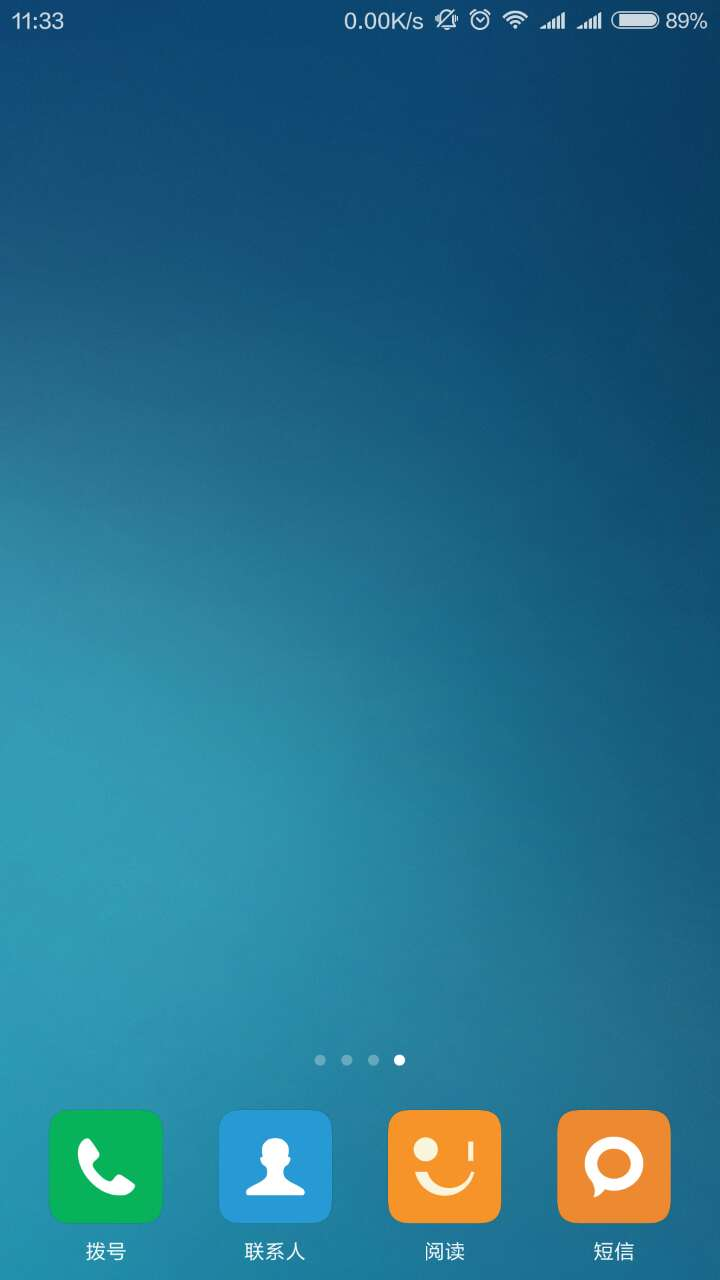
\includegraphics[height=0.3\textheight]{./figure/desktop-3.jpg}
    \end{center}

    大理寺少卿孙以为不然,生活宜随性起浪,手机桌面亦应如是,show 之。

    \begin{center}
    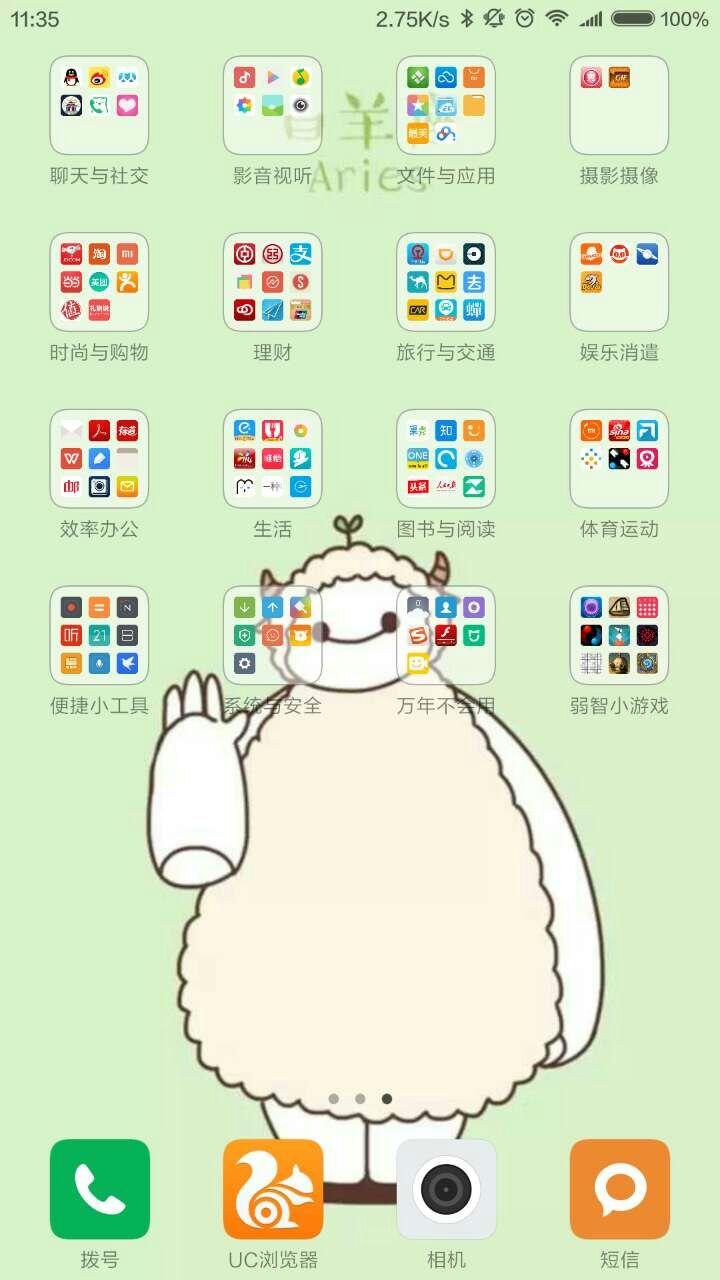
\includegraphics[height=0.3\textheight]{./figure/desktop-4.jpg}
    \end{center}

    钦天监监正冷冷笑数声,“泯然众人,不识天行有常,天机无常。” Show 其手机桌面,红点纷飞,内阁诸强迫症皆吐血数升,俯拜天道。

    \begin{center}
    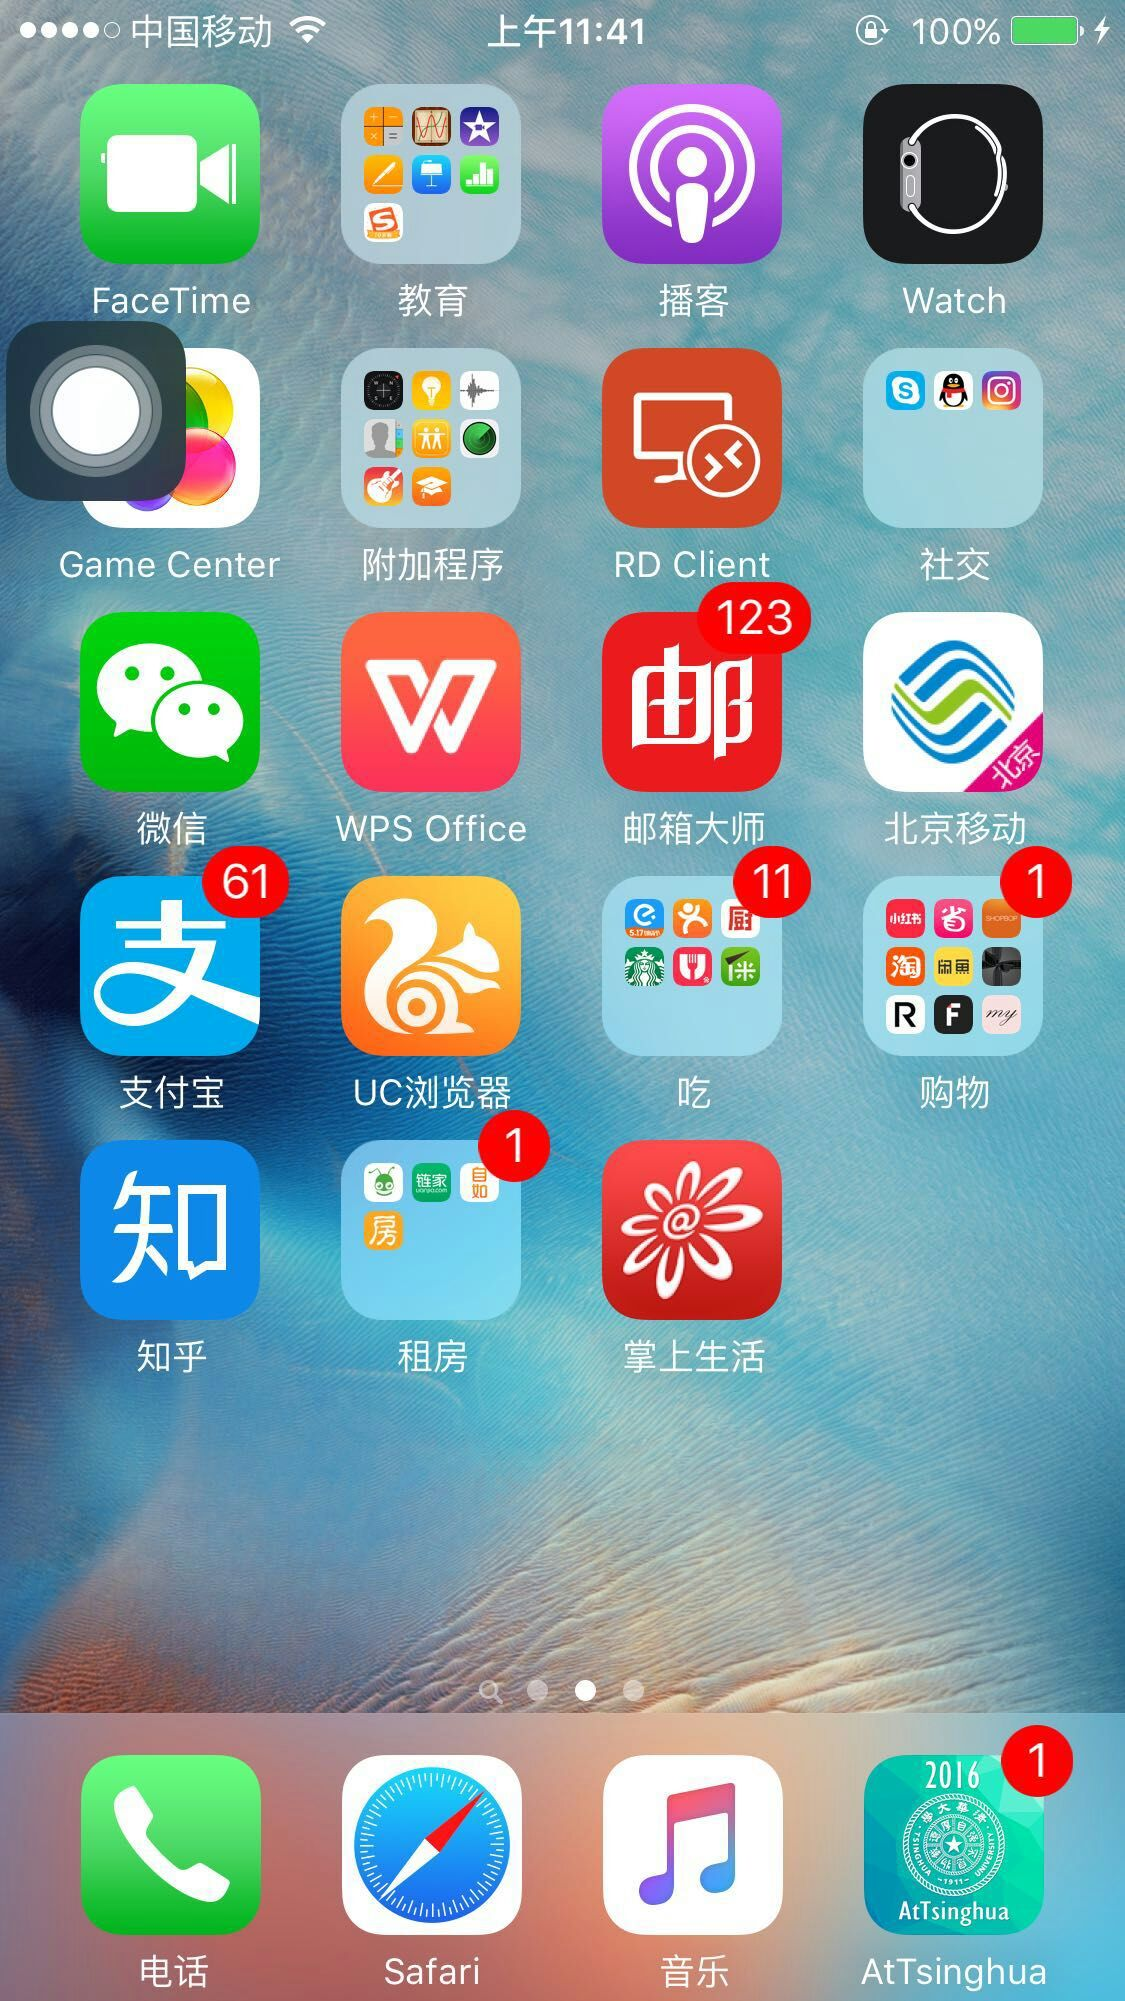
\includegraphics[height=0.3\textheight]{./figure/desktop-5.jpg}
    \end{center}

    国子监监正李淡然,“返璞归真,清水芙蓉,方为教化真意。”

    \begin{center}
    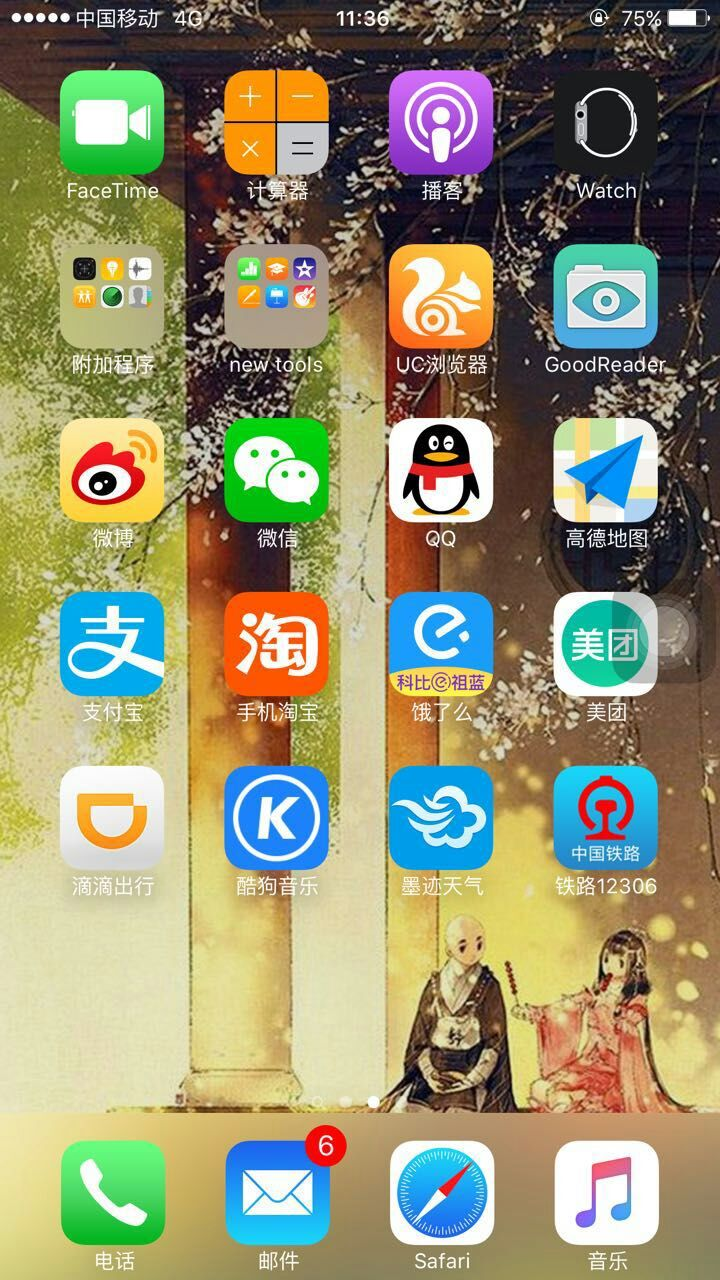
\includegraphics[height=0.3\textheight]{./figure/desktop-6.jpg}
    \end{center}

    锦衣卫都指挥使白默然,“兵者,国之重器,死生之道,不可轻以示人。”

    礼部侍郎魏叹曰,“争奇斗艳,毫无大夫气度,非礼也,非礼也。”

    \appendix

    %!Mode::"TeX:UTF-8"

\chapter{七葫大事记}

\begin{itemize}
    \item{2016年7月5日,经小明王朝执行内阁提案,内阁首辅、XX殿大学士袁票拟批蓝,《七葫拍案惊奇》创作计划启动。}
\end{itemize}


\end{CJK}
\end{document}

